\chapter{Phát biểu bài toán}

\section{Mục tiêu nghiên cứu}
Bài toán được thực hiện không chỉ dừng lại ở nhiệm vụ nhận diện khuôn mặt cơ bản mà đi sâu vào đánh giá định lượng (Quantitative Evaluation) hiệu năng của mô hình trước tác động của thời gian. Các mục tiêu cụ thể bao gồm:

\begin{enumerate}
    \item \textbf{Kiểm chứng "Nghịch lý tuổi tác":} Trước đây, các nghiên cứu trên các đặc trưng thủ công (hand-crafted features) thường cho rằng người già dễ nhận diện hơn do cấu trúc khuôn mặt ổn định. Bài toán này tập trung chứng minh thực tế ngược lại đối với các mô hình Deep CNN hiện đại: độ chính xác nhận diện thường thấp hơn ở nhóm người cao tuổi do sự suy giảm chất lượng phân phối giả mạo (impostor distribution).
    
    \item \textbf{Đo lường sự suy giảm hiệu năng (Degradation Rate):} Tính toán và định lượng mức độ giảm sút của độ chính xác nhận diện khi khoảng cách thời gian (Time Gap) giữa hai lần chụp tăng dần (theo các mốc 2, 4, 6, 8, 10 năm).
    
    \item \textbf{So sánh tính bền vững của các hàm Loss:} Đánh giá hiệu quả của cơ chế "Biên thích ứng" (Adaptive Margin) trong MagFace so với cơ chế "Biên cố định" (Fixed Margin) trong ArcFace khi xử lý dữ liệu có độ chênh lệch tuổi tác lớn, từ đó rút ra các nhận định về hướng tối ưu hóa mô hình.
\end{enumerate}

\section{Đặc tả Input và Output}
Để giải quyết các mục tiêu trên, hệ thống thực nghiệm được thiết kế với luồng dữ liệu như sau:
\begin{figure}[H] 
    \centering
    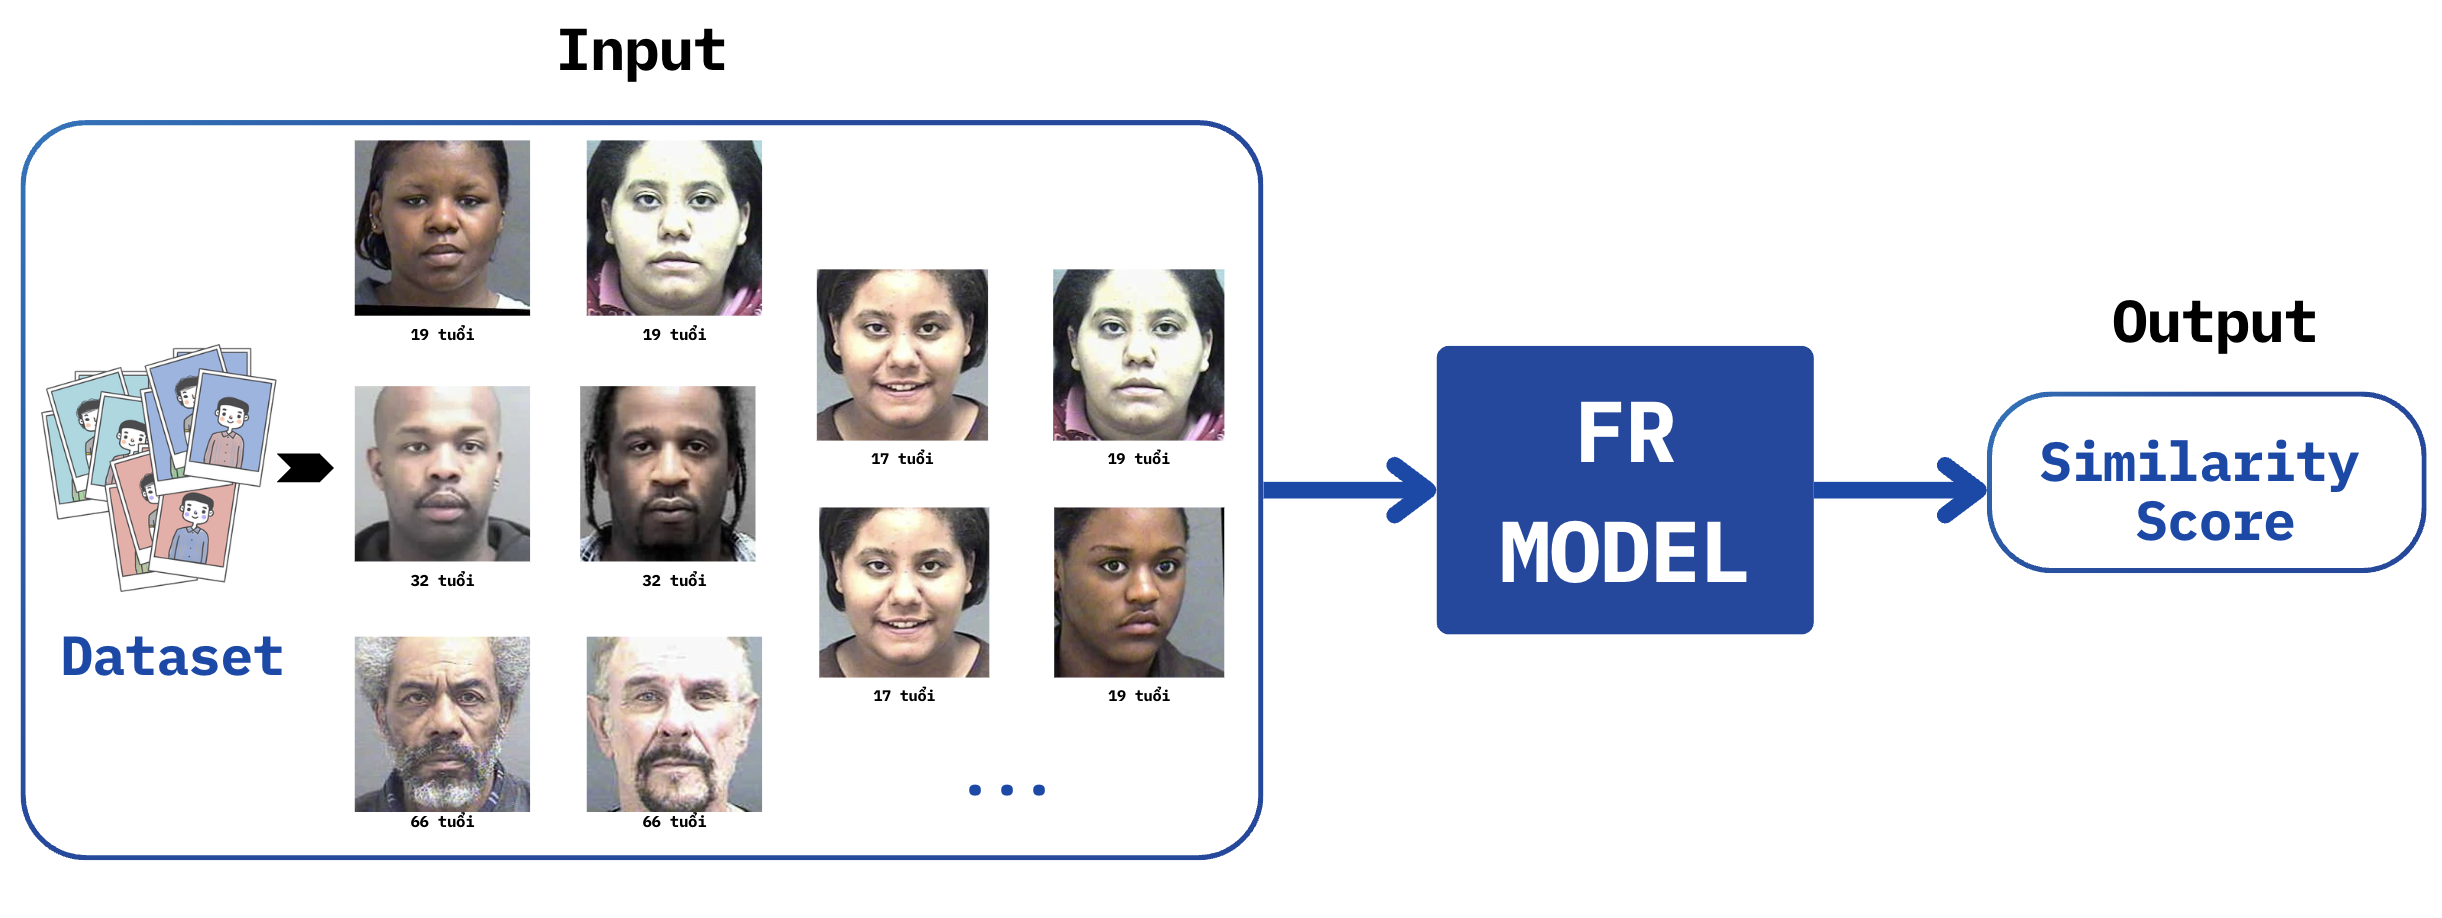
\includegraphics[width=0.8\linewidth]{logos/3.png} 
    \caption{Input và Output của bài toán}
\end{figure}
\subsection{Đầu vào (Input)}
Đơn vị xử lý cơ bản của hệ thống là \textbf{một cặp ảnh khuôn mặt (a pair of face images)} đã được tiền xử lý cắt và căn chỉnh (aligned). Các cặp ảnh này được phân loại kỹ lưỡng dựa trên các thuộc tính:
\begin{itemize}
    \item \textbf{Loại cặp ảnh:}
    \begin{itemize}
        \item \textit{Genuine (Positive):} Cặp ảnh của cùng một người tại hai thời điểm khác nhau.
        \item \textit{Impostor (Negative):} Cặp ảnh của hai người khác nhau.
    \end{itemize}
    \item \textbf{Nhóm tuổi:} Dữ liệu được chia thành 3 nhóm chính để so sánh đặc tính:
    \begin{itemize}
        \item Nhóm Trẻ (Young): 16 - 29 tuổi.
        \item Nhóm Trung niên (Middle-aged): 30 - 49 tuổi.
        \item Nhóm Cao tuổi (Senior): 50 - 70 tuổi.
    \end{itemize}
    \item \textbf{Khoảng cách thời gian (Time Gap):} Các cặp ảnh Genuine được lựa chọn sao cho độ chênh lệch thời gian chụp lần lượt là 2, 4, 6, 8 và 10 năm.
\end{itemize}

\subsection{Đầu ra (Output)}
Từ dữ liệu đầu vào, hệ thống thực hiện trích xuất đặc trưng và tính toán để đưa ra:
\begin{itemize}
    \item \textbf{Kết quả trực tiếp:} Một giá trị điểm tương đồng (\textit{Similarity Score}) cho mỗi cặp ảnh, được tính bằng độ tương tự Cosine (Cosine Similarity) giữa hai vector đặc trưng.
    \item \textbf{Kết quả phân tích:} Từ tập hợp điểm số của hàng ngàn cặp ảnh, bài toán xây dựng các biểu đồ phân phối điểm (Score Distribution), đường cong ROC và tính toán các chỉ số đánh giá chất lượng hệ thống như Độ chính xác (Accuracy), Tỷ lệ lỗi cân bằng (EER - Equal Error Rate), và Tỷ lệ xác thực đúng tại tỷ lệ chấp nhận sai (TAR@FAR).
\end{itemize}



\section{Phạm vi và Phương pháp thực nghiệm}
Bài toán được giới hạn và thực nghiệm trên các tập dữ liệu chuẩn có gán nhãn tuổi chính xác (như MORPH-II hoặc AgeDB-30). 

Phương pháp luận chính là so sánh đối chứng (benckmarking) giữa hai mô hình đại diện cho trạng thái hiện tại (SOTA):
\begin{itemize}
    \item \textbf{ArcFace:} Đại diện cho nhóm phương pháp sử dụng hàm mất mát với biên góc cố định (Fixed Margin Loss).
    \item \textbf{MagFace:} Đại diện cho nhóm phương pháp mới sử dụng biên thích ứng dựa trên chất lượng ảnh (Quality-aware Adaptive Margin Loss).
\end{itemize}
Việc so sánh này nhằm làm rõ sự khác biệt về tính bền vững của từng phương pháp tiếp cận khi đối mặt với thách thức lão hóa khuôn mặt.